\documentclass{article}

% enable these lines below while using overleaf, disable for texmaker/latex workshop
%\usepackage[utf8]{inputenc}
%\usepackage{stmaryrd}
%\usepackage{algorithm,algpseudocode} 
%\usepackage{galois}

\usepackage{xspace}
\usepackage{amsmath}
\usepackage{afterpage}
\usepackage{graphicx,lipsum}   
\usepackage{figlatex,wrapfig}
\usepackage[dvipsnames]{xcolor}
\usepackage{listings,amssymb,mathtools}
\usepackage{mathrsfs}
\usepackage{array,multirow}
\usepackage{pifont}
\usepackage{caption}
\usepackage{geometry}
\usepackage{textcomp}

\usepackage{tikz}
\usepackage[shortlabels]{enumitem}

% for colours
\usepackage{xspace}
\usepackage[colorlinks]{hyperref}
\hypersetup{
	colorlinks = true,
	citecolor = {violet},
	linkcolor = {blue},
	urlcolor  = {blue}
}

% for arrow diagrams
\usepackage{amsmath}
\usepackage{amssymb}
\usepackage{smartdiagram}
\usepackage{tikz}
\usetikzlibrary{arrows,positioning}

\usepackage[parfill]{parskip}

% for bib handline
\usepackage[numbers]{natbib}
\usepackage{url}

\newcommand{\mosc}{\texttt{memory\_order\_seq\_cst}\xspace}
\newcommand{\moacqrel}{\texttt{memory\_order\_acq\_rel}\xspace}
\newcommand{\morel}{\texttt{memory\_order\_release}\xspace}
\newcommand{\moacq}{\texttt{memory\_order\_acquire}\xspace}
\newcommand{\mocon}{\texttt{memory\_order\_consume}\xspace}
\newcommand{\morlx}{\texttt{memory\_order\_relaxed}\xspace}

\newcommand{\seqb}[2]{{#1} {\color{Blue}$\rightarrow^{sb}$} \color{black}{#2} }
\newcommand{\sw}[2]{{#1} {\color{Blue}$\rightarrow^{sw}$} \color{black}{#2} }
\newcommand{\hb}[2]{{#1} {\color{Blue}$\rightarrow^{hb}$} \color{black}{#2}}
\newcommand{\rf}[2]{{#1} {\color{Blue}$\rightarrow^{rf}$} {#2} }
\newcommand{\too}[2]{{#1} {\color{Blue}$\rightarrow^{to}$} {#2} }
\newcommand{\mo}[2]{{#1} {\color{Blue}$\rightarrow^{mo}$} {#2} }

\newcommand{\var}[1]{\color{OliveGreen}\texttt{#1}\color{black}}
\newcommand{\fun}[2]{\color{Sepia}\texttt{#1(\color{Gray}\textit{#2}\color{Sepia})}\color{black}}
\newcommand{\class}[1]{\color{DarkOrchid}\texttt{#1}\color{black}}

\title{fence-synthesis-paper}
\date{}

\begin{document}

\maketitle
\textit{\textbf{Abstract-}}

\section{Introduction} \label{sec:intro}
% ------------ INTRO PARAS ------------------
\par
A programmer working with relaxed memory constraints would want all the advantages of the relaxed model - such as speed and concurrency. However, using relaxed memory constraints comes with its own issues. In relaxed memory models, memory operations such as \textit{reads} and \textit{writes} can be reordered in order to achieve these properties. These instruction reorderings can cause certain variables to have different values in different execution runs of the same program, hence resulting in behaviour which is unexpected or surprising. These include not behaving according to sequentially consistent standards, or outputting unexpected values of variables.

\par
In this project, we suggest an approach to prevent certain unexpected behaviour, such as unexpected outputs due to concurrent instruction re-orderings in the C11 relaxed model.

\par
To tackle this, the programmer may add \textit{"assert"} statements in the source code, which will check that certain properties remain unchanged in each run of the program, such as the value of a variable in a certain thread. Each program will have several possibilities of runs where instructions will be executed in different orders. In some of these runs, there might be cases where the assertion does not hold and it gets violated. In the case that the \textit{assert} statement gets violated, the program execution will stop. The object of this project is to insert a minimum number of \textbf{C11 fences} in the source code of the program at the right places so that these assertions are satisfied and do not get violated.

% -------------------- MOTIVATION E.G. ------------------------
\subsection{Motivation Example}

% -------------------- FIG 1: BASIC ------------------------
\begin{figure}[!htb]
\begin{center}
\texttt{
init y := 0, x := 0;\\
	\begin{tabular}{c l || c l}
		(1) & y := 1 & (5) & x := 1\\
		(2) & if x == 0 & (6) & if y == 0\\
		(3) & \qquad c := 1 & (7) & \qquad c := 0\\
		(4) & \qquad t = c \color{olive}//1 & (8) & \qquad t = c \color{olive}//0
	\end{tabular}
}
	\caption{Simple two-thread dekker program}\label{fig:dekker1}
\end{center}
\end{figure}
\ishComment{to use R, W here as well? to show atomic operations? to use brackets for if?}

\par
In a sequentially consistent model, the multi-threaded program in Fig \ref{fig:dekker1} would execute the instructions in a sequentially consistent order. The final values read by variable \textit{t} would be 1 and 0 for each thread respectively. Therefore it can be said that the ``output'' would always be ``10''. However, in the case of a relaxed model, such as in a C11/C++11 program when all the instructions are relaxed, reading outputs of ``00'', ``01'', ``11'' may even be possible, thereby violating the rules of sequential consistency. Such an output may or may not be unexpected for the programmer, depending upon their requirements.

\par
For this reason, the programmer needs to provide their requirements about what values are expected at which locations by specifying a local safety property.

% --------------- FIG 2.2 basic + assert -------------
\begin{figure}[!htb]
\begin{center}
\texttt{
init y := 0, x := 0;\\
	\begin{tabular}{c l || c l}
		(1) & W$\mathtt{_{rel}}$y(1) & (5) & W$\mathtt{_{rel}}$x(1)\\
		(2) & if R$\mathtt{_{rel}x}$ == 0 & (6) & if R$\mathtt{_{rel}y}$ == 0\\
		(3) & \qquad W$\mathtt{_{rel}}$c(1) & (7) & \qquad W$\mathtt{_{rel}}$c(0)\\
		(4) & \qquad assert($\mathtt{R_{rel}c}$ == 1) & (8) & \qquad assert($\mathtt{R_{rel}c}$ == 0)
	\end{tabular}
}
	\caption{Simple two-thread dekker program in C11 syntax with assertions}\label{fig:dekker2}
\end{center}
\end{figure}

\par
Such a specification may be made in the form of assertions such as those described in Fig \ref{fig:dekker2} This ``assert'' statement checks that the expression provided to it holds at that point in the program. At the end of the threads, this safety property might not be satisfied. In this case, the program stops or exits, giving an error output. The objective of the tool to be created is to prevent the program from exhibiting behaviour which is unexpected for the programmer, hence preventing the error output as well as ensuring the provided specifications. For the purposes of this paper, we require the safety property to be specified as assertions in the program.

\section{Our Approach}
Given a buggy input program $P$, \ourtechnique attempts to 
stop the buggy traces or counter examples (traces with 
assert statement violations) of $P$ by inserting \cc fences.
%
To do so the technique must accomplish three objectives
(O1) determine whether the buggy trace can be stopped by 
synthesizing \cc fences,
(O2) determine the placement of optimal number of synthesized 
fences (\ie the least number of program locations where fences 
must be synthesized that is sufficient to stop the trace), 
and
(O3) determine the optimal memory order of the synthesized 
fences (\ie the weakest memory order of synthesized fences 
that is sufficient to stop the trace).
%
We present the \ourtechnique-algorithm (Algorithm
\ref{alg:main algo}) that realizes the three objectives.
The algorithm takes a \cc program as input
and determines the optimal fence placement that can stop
the buggy traces of the input program or determines that
the program cannot be made bug-free with \cc fences.

\begin{algorithm}[h]
	\caption{Fence Synthesis}
	\label{alg:main algo}
	\DontPrintSemicolon
	\SetAlgoLined
	
	\SetKwFunction{Fmain}{\ourtechnique}
	\SetKwFunction{Fceg}{generateCounterExamples}
	\SetKwFunction{FcandidateF}{candidateFences}
	\SetKwFunction{Frel}{computeRelations}
	\SetKwFunction{Fwk}{weakFensying}
	\SetKwFunction{Fst}{strongFensying}
	\SetKwFunction{Fmin}{minModel}
	
	\SetKwData{satquery}{$\Phi$}
	\SetKwData{ce}{CE}
	\SetKwData{wk}{weakCycles}
	\SetKwData{st}{strongCycles}
	
	\SetKwProg{Fn}{Function}{:}{}
	
	\Fn{\Fmain{input program $P$}}{		
		\satquery $:=$ $\top$\;
		\ce $:=$ \Fceg{$P$}\;
		\ForAll(\tcc*[f]{$\tau = \langle \events_\tau, \setHB, \setMO, \setRF \rangle$}) {$\tau \in$ \ce}{
			$\events_{\imm{\tau}}$ $:=$ $\events_\tau$ $\union$ \FcandidateF{$\tau$}\;
			$(\hb{\imm{\tau}}{}{}, \mo{\imm{\tau}}{}{}, \rf{\imm{\tau}}{}{}, \rfinv{\imm{\tau}}{}{}, \fr{\imm{\tau}}{}{})$ 
				$:=$ \Frel{$\tau,\events_{\imm{\tau}}$}\;
			\wk $:=$ \Fwk{$\imm{\tau}$}\;
			\st $:=$ \Fst{$\imm{\tau}$}\;
			\If{\wk $= \emptyset$ $\^$ \st $= \emptyset$} {
				\KwRet $\emptyset$
				\tcc*{cannot stop $\tau$}
			}			
		}
	
		\satquery $:=$ \satquery $\^$ $\formula{$\wk $\v$ \st$}$\;
		\KwRet \Fmin{\satquery}
	}
		
		
%		\State 
%		\State $ \seqb{\imm{\tau}}{}{} := $ computeSB($\setSB, \events_{\imm{\tau}}$) \State $ \so{\tau^{\mathtt{im}}}{}{} := $ computeSO($\events_{\imm{\tau}}, \setHB, \setMO, \setRF, \seqb{\imm{\tau}}{}{}$)
%		\State cycles := computeCycles($ \so{\imm{\tau}}{}{} $)
%		\If {cycles == $ \emptyset $}
%		\State \texttt{Abort} (``This trace can't be stopped using \cc fences.'')
%		\State \Return
%		\EndIf
%		\State $\phi := \phi\ \^ \formula{\so{\imm{\tau}}{}{}} $ 
%		%			\State $ \phi := \phi_\tau $
%		\EndFor
%		\State F:= MinModel($ \phi $)
%		\State \Return F



%		% no enabled events left ie maximal sequence explored
%		\lIf{\FunexploredEv{$\tau$} = $\emptyset$}{\KwRet 
%			\tcc*[f]{maximal sequence explored}}
%		
%		% if there is no sequence and no constraint sequence
%		\If(\tcc*[f]{find next event to explore}){$S = \emptysequence$}{
%			\If(\tcc*[f]{multiple leads possible}){
%				$\exists (e_r, e_w) \in$ \FunexploredRW{$\tau, F$}}{
%				\lForAll{$e_w' \in \ui{\tau}{F}{e_r}$}{
%					\Fupdate($\tau, e_w', F$)
%				}
%				\nexte := $e_r$
%			}
%			\lElse{
%				\nexte := any event $\in$ \FunexploredEv{$\tau$};
%			}
%			
%			% updateLeads wrt to selected event
%			\Fupdate($\tau$, \nexte, $F$)
%		}
%		
%		% there is a sequence to be explored
%		\lElse{
%			\nexte := $\hd{S}$
%		}
%		
%		%		\lIf(\tcc*[f]{if no branch explore \nexte})
%		\lIf
%		{$S = \emptysequence \^$ \FunexploredLd{$\tau$} = $\emptyset$}{
%			$\ld{\s{\tau}} \cunioneq (\emptysequence,\ \seq{${\nexte}$},\ F)$
%		}
%		
%		\lElseIf(\tcc*[f]{explore next event in $S$}){$S \neq \emptysequence$}{
%			$\ld{\s{\tau}} \cunioneq (\emptysequence,\ S,\ F)$
%		}
%		
%		\While(\tcc*[f]{explore all leads})
%		{$\exists l \in$ \FunexploredLd{$\tau$}}{
%			\nextseq := $l^s \cmerge l^c$\;
%			\Dprime := $\{\tau' \| \hd{${\nextseq}$}.\tau' \in Dn(\s{\tau})\}$\;
%			\Fexplore{$\tau.\hd{${\nextseq}$},\ \tl{${\nextseq}$}$, \Dprime, $l^F$}\;
%			$\dn{\s{\tau}} \unioneq$ \nextseq
%		}
%	}
\end{algorithm}
\divComment{Can we give termination guarantee?}

\noindent
{\bf Algorithm~\ref{alg:main algo} overview:} 
The algorithm assumes the knowledge of the set of counter
examples in the form of traces (\ie a set of events and 
the sets of relations on the events, as defined in Section
\ref{sec:preliminaries}).
%
Broadly the algorithm places candidate fences before and
after every program event then works towards eliminating 
fences that do not contribute to the optimal solution.
%
The elimination is a two-phase process where in the first
phase the algorithm discards candidate fences that do not 
contribute to the violation of either a coherence condition 
or the \sc total order. 
Further, in the second phase the algorithm reduces the 
remaining candidate fences to the optimal number with
the optimal memory order.

The algorithm takes a \cc program as input and relies on a 
counter example generator to return the set of counter 
examples or buggy traces of the input program (line 3).
It then transforms the buggy traces $\tau$ to an intermediate 
trace $\imm{\tau}$ by synthesizing candidate 
fences (lines 5,6).
%
The algorithm iterates over each counter example to 
collect cycles in coherence conditions or \sc total order
(lines 7,8) and aborts the process if for any buggy trace
the set of cycles is empty indicating the trace cannot be 
stopped by synthesizing \cc fences (lines 9,10).
This step constitutes the phase one where any fence not
involved in a cycle is discarded.
%
On the fences involved in the discovered cycles, we use a
SAT solver to compute the minimum number of fences
(line 11,12). 
%
The fences that contribute to the optimal (in number of
fences) set of of fences are then mapped back to their 
corresponding cycle to ascertain the memory order of 
the fence.
%
This step along with the previous step using a SAT solver
performs the phase two of elimination of candidate fences.
%
The final form of the buggy trace (with the optimal 
synthesized fences) renders the trace invalidated,
represented as $\inv{\tau}$, ensuring that the trace 
does not belong to the set of traces of the transformed
(fixed) program $\fx{P}$. 
%
We discuss the details of each step below.

\noindent
{\bf Counter examples and candidate fences:}
\ourtechnique is a fence synthesis technique to stop
buggy traces that requires a set of buggy traces to 
perform its analysis. We thus rely on an external counter
example generator that takes the input program $P$ and
returns the set of buggy traces (line 3) where each buggy 
trace is a tuple $\langle \events_\tau, \setHB, \setMO, 
\setRF \rangle$.
%
Consider the \hlref{mutex-input-program} where two 
threads are racing to mutually exclusively update the
value of $x$. The program under \cc violates the 
mutual exclusion property and a counter example generator
returns two buggy traces diagrammatically represented in
\hlref{mutex-bt1} and \hlref{mutex-bt2}.

\begin{figure}[!htb]
	\begin{center}
		\setlength{\tabcolsep}{5pt}
		\begin{tabular}{|l||l|}
			\hline
			\multicolumn{2}{|c|}{Initially: $Flag_1=0, Flag_2 = 0, x=0$} \\
			
			$ Flag_1 :=_\rlx 1 $ & $ Flag_2 :=_\rlx 1  $ \\
			\textbf{if} $ (Flag_2 =_\rlx 0) $ & \textbf{if} $ (Flag_1 =_\rlx 0) $ \\
			\quad $ x :=_\rlx 1 $ & \quad $ x :=_\rlx 2 $ \\
			\quad assert($ x =_\rlx 1 $) & \quad assert($ x =_\rlx 2 $) \\
			\hline
			
			\multicolumn{2}{c}{\hl{mutex-input-program}}
		\end{tabular} 
	\end{center}
\end{figure}

\begin{figure}[!h]
	\begin{tabular}{|c|c|c|c|}
		\hline
		\resizebox{0.24\textwidth}{!}{\tikzset{every picture/.style={line width=0.75pt}} %set default line width to 0.75pt        
\begin{tikzpicture}[x=1em,y=1em,yscale=-1,xscale=-1]
	\tikzstyle{every node}=[font=\normalfont]
	
	\node (ifl1) [inner sep=2pt,color=Brown] {$\mathbb{I}(Flag_1,0)$};
	\node (ifl2) [right=30pt,inner sep=2pt,color=Brown] {$\mathbb{I}(Flag_2,0)$};
	
	\node (f11) [below left=10pt and -30pt of ifl1,inner sep=2pt, color=White] {$\mathbb{F}_{11}$};
	\node (fl1) [below=10pt of f11, inner sep=2pt] {$ W^\sc(Flag_1,1) $};
	\node (f12) [below=10pt of fl1, inner sep=2pt, color=White] {$\mathbb{F}_{12}$};
	\node (rfl2) [below=10pt of f12, inner sep=2pt] {$R^\rlx(Flag_2,0)$:};
	\node (f13) [below=10pt of rfl2, inner sep=2pt, color=White] {$\mathbb{F}_{13}$};
	\node (cs11) [below=10pt of f13, inner sep=2pt] {$ W^\rlx(x,1) $};
	\node (f14) [below=10pt of cs11, inner sep=2pt, color=White] {$\mathbb{F}_{14}$};
	\node (cs12) [below=10pt of f14, inner sep=2pt] {$ R^\rlx(x,1) $};
	\node (f15) [below=10pt of cs12, inner sep=2pt, color=White] {$\mathbb{F}_{15}$};
	
	\node (f21) [right=50pt of f11, inner sep=2pt, color=White] {$\mathbb{F}_{21}$};
	\node (fl2) [below=10pt of f21, inner sep=2pt] {$W^\sc(Flag_2,1)$};
	\node (f22) [below=10pt of fl2, inner sep=2pt, color=White] {$\mathbb{F}_{22}$};
	\node (rfl1) [below=10pt of f22, inner sep=2pt] {$R^\rlx(Flag_1,0)$:};
	\node (f23) [below=10pt of rfl1, inner sep=2pt, color=White] {$\mathbb{F}_{23}$};
	\node (cs21) [below=10pt of f23, inner sep=2pt] {$ W^\rlx(x,2) $};
	\node (f24) [below=10pt of cs21, inner sep=2pt, color=White] {$\mathbb{F}_{24}$};
	\node (cs22) [below=10pt of f24, inner sep=2pt] {$ R^\rlx(x,1) $};
	\node (f25) [below=10pt of cs22, inner sep=2pt, color=White] {$\mathbb{F}_{23}$};
	%
	\draw [->,>=stealth,color=RedOrange] ($ (ifl1.south east)+(0.8,-5pt) $) -- node[pos=0.3,left=-2pt,font=\scriptsize,color=black] { $\lmo$ } ($ (fl1.north east)+(1.2,-5pt) $);
	\draw [->,>=stealth,color=RedOrange] ($ (ifl2.south west)+(-1.2,-5pt) $) -- node[pos=0.3,right=-2pt,font=\scriptsize,color=black] { $\lmo$ } ($ (fl2.north west)+(-0.7,-5pt) $);
	
	\draw [->,>=stealth,color=PineGreen] ($ (ifl1.south east)+(0.8,-5pt) $) -- node[pos=0.8,right=-2pt,font=\scriptsize,color=black] { $\lrf$ } ($ (rfl1.north west)+(-1.2,-5pt) $);
	\draw [->,>=stealth,color=PineGreen] ($ (ifl2.south west)+(-1.2,-5pt) $) -- node[pos=0.8,left=-2pt,font=\scriptsize,color=black] { $\lrf$ } ($ (rfl2.north east)+(1.2,-5pt) $);
	
	\draw [->,>=stealth,color=RedOrange] (cs21)  -- node[midway,above=-2pt,font=\scriptsize,color=black] { $\lmo$ } (cs11);
	\draw [->,>=stealth,color=PineGreen] (cs11)  -- node[midway,above=-2pt,font=\scriptsize,color=black] { $\lrf$ } (cs22);
	\draw [->,>=stealth,color=PineGreen] ($ (cs11.south)+(10.4pt,0) $)  -- node[midway,left=-2pt,font=\scriptsize,color=black] { $\lrf$ } ($ (cs12.north)+(10.4pt,0) $);
	
	\draw [->,>=stealth,color=CarnationPink] (fl1)  -- node[midway,right=-2pt,font=\scriptsize,color=black] { $\lsb$ } (rfl2);
	\draw [->,>=stealth,color=CarnationPink] (rfl2) -- node[midway,right=-2pt,font=\scriptsize,color=black] { $\lsb$ } (cs11);
	\draw [->,>=stealth,color=CarnationPink] (cs11) -- node[midway,right=-2pt,font=\scriptsize,color=black] { $\lsb$ } (cs12);
	
	\draw [->,>=stealth,color=CarnationPink] (fl2)  -- node[midway,right=-2pt,font=\scriptsize,color=black] { $\lsb$ } (rfl1);
	\draw [->,>=stealth,color=CarnationPink] (rfl1) -- node[midway,right=-2pt,font=\scriptsize,color=black] { $\lsb$ } (cs21);
	\draw [->,>=stealth,color=CarnationPink] (cs21) -- node[midway,right=-2pt,font=\scriptsize,color=black] { $\lsb$ } (cs22);
	
\end{tikzpicture}
} &
		\resizebox{0.24\textwidth}{!}{\tikzset{every picture/.style={line width=0.75pt}} %set default line width to 0.75pt        
\begin{tikzpicture}[x=1em,y=1em,yscale=-1,xscale=-1]
	\tikzstyle{every node}=[font=\normalfont]
	
	\node (ifl1) [inner sep=2pt,color=Brown] {$\mathbb{I}(Flag_1,0)$};
	\node (ifl2) [right=30pt,inner sep=2pt,color=Brown] {$\mathbb{I}(Flag_2,0)$};
	
	\node (f11) [below left=10pt and -30pt of ifl1,inner sep=2pt] {$\mathbb{F}_{11}$};
	\node (fl1) [below=10pt of f11, inner sep=2pt] {$ W^\sc(Flag_1,1) $};
	\node (f12) [below=10pt of fl1, inner sep=2pt] {$\mathbb{F}_{12}$};
	\node (rfl2) [below=10pt of f12, inner sep=2pt] {$R^\rlx(Flag_2,0)$:};
	\node (f13) [below=10pt of rfl2, inner sep=2pt] {$\mathbb{F}_{13}$};
	\node (cs11) [below=10pt of f13, inner sep=2pt] {$ W^\rlx(x,1) $};
	\node (f14) [below=10pt of cs11, inner sep=2pt] {$\mathbb{F}_{14}$};
	\node (cs12) [below=10pt of f14, inner sep=2pt] {$ R^\rlx(x,1) $};
	\node (f15) [below=10pt of cs12, inner sep=2pt] {$\mathbb{F}_{15}$};
	
	\node (f21) [right=50pt of f11, inner sep=2pt] {$\mathbb{F}_{21}$};
	\node (fl2) [below=10pt of f21, inner sep=2pt] {$W^\sc(Flag_2,1)$};
	\node (f22) [below=10pt of fl2, inner sep=2pt] {$\mathbb{F}_{22}$};
	\node (rfl1) [below=10pt of f22, inner sep=2pt] {$R^\rlx(Flag_1,0)$:};
	\node (f23) [below=10pt of rfl1, inner sep=2pt] {$\mathbb{F}_{23}$};
	\node (cs21) [below=10pt of f23, inner sep=2pt] {$ W^\rlx(x,2) $};
	\node (f24) [below=10pt of cs21, inner sep=2pt] {$\mathbb{F}_{24}$};
	\node (cs22) [below=10pt of f24, inner sep=2pt] {$ R^\rlx(x,1) $};
	\node (f25) [below=10pt of cs22, inner sep=2pt] {$\mathbb{F}_{23}$};
	%
	\draw [->,>=stealth,color=RedOrange] ($ (ifl1.south east)+(0.8,-5pt) $) -- node[pos=0.3,left=-2pt,font=\scriptsize,color=black] { $\lmo$ } ($ (fl1.north east)+(1.2,-5pt) $);
	\draw [->,>=stealth,color=RedOrange] ($ (ifl2.south west)+(-1.2,-5pt) $) -- node[pos=0.3,right=-2pt,font=\scriptsize,color=black] { $\lmo$ } ($ (fl2.north west)+(-0.7,-5pt) $);
	
	\draw [->,>=stealth,color=PineGreen] ($ (ifl1.south east)+(0.8,-5pt) $) -- node[pos=0.8,right=-2pt,font=\scriptsize,color=black] { $\lrf$ } ($ (rfl1.north west)+(-1.2,-5pt) $);
	\draw [->,>=stealth,color=PineGreen] ($ (ifl2.south west)+(-1.2,-5pt) $) -- node[pos=0.8,left=-2pt,font=\scriptsize,color=black] { $\lrf$ } ($ (rfl2.north east)+(1.2,-5pt) $);
	
	\draw [->,>=stealth,color=RedOrange] (cs21)  -- node[midway,above=-2pt,font=\scriptsize,color=black] { $\lmo$ } (cs11);
	\draw [->,>=stealth,color=PineGreen] (cs11)  -- node[midway,above=-2pt,font=\scriptsize,color=black] { $\lrf$ } (cs22);
	\draw [->,>=stealth,color=PineGreen] ($ (cs11.south)+(10.4pt,0) $)  -- node[midway,left=-2pt,font=\scriptsize,color=black] { $\lrf$ } ($ (cs12.north)+(10.4pt,0) $);
	
	\draw [->,>=stealth,color=CarnationPink] (f11)  -- node[midway,right=-2pt,font=\scriptsize,color=black] { $\lsb$ } (fl1);
	\draw [->,>=stealth,color=CarnationPink] (fl1)  -- node[midway,right=-2pt,font=\scriptsize,color=black] { $\lsb$ } (f12);
	\draw [->,>=stealth,color=CarnationPink] (f12)  -- node[midway,right=-2pt,font=\scriptsize,color=black] { $\lsb$ } (rfl2);
	\draw [->,>=stealth,color=CarnationPink] (rfl2) -- node[midway,right=-2pt,font=\scriptsize,color=black] { $\lsb$ } (f13);
	\draw [->,>=stealth,color=CarnationPink] (f13)  -- node[midway,right=-2pt,font=\scriptsize,color=black] { $\lsb$ } (cs11);
	\draw [->,>=stealth,color=CarnationPink] (cs11) -- node[midway,right=-2pt,font=\scriptsize,color=black] { $\lsb$ } (f14);
	\draw [->,>=stealth,color=CarnationPink] (f14)  -- node[midway,right=-2pt,font=\scriptsize,color=black] { $\lsb$ } (cs12);
	\draw [->,>=stealth,color=CarnationPink] (cs12) -- node[midway,right=-2pt,font=\scriptsize,color=black] { $\lsb$ } (f15);
	
	\draw [->,>=stealth,color=CarnationPink] (f21)  -- node[midway,right=-2pt,font=\scriptsize,color=black] { $\lsb$ } (fl2);
	\draw [->,>=stealth,color=CarnationPink] (fl2)  -- node[midway,right=-2pt,font=\scriptsize,color=black] { $\lsb$ } (f22);
	\draw [->,>=stealth,color=CarnationPink] (f22)  -- node[midway,right=-2pt,font=\scriptsize,color=black] { $\lsb$ } (rfl1);
	\draw [->,>=stealth,color=CarnationPink] (rfl1) -- node[midway,right=-2pt,font=\scriptsize,color=black] { $\lsb$ } (f23);
	\draw [->,>=stealth,color=CarnationPink] (f23)  -- node[midway,right=-2pt,font=\scriptsize,color=black] { $\lsb$ } (cs21);
	\draw [->,>=stealth,color=CarnationPink] (cs21) -- node[midway,right=-2pt,font=\scriptsize,color=black] { $\lsb$ } (f24);
	\draw [->,>=stealth,color=CarnationPink] (f24)  -- node[midway,right=-2pt,font=\scriptsize,color=black] { $\lsb$ } (cs22);
	\draw [->,>=stealth,color=CarnationPink] (cs22) -- node[midway,right=-2pt,font=\scriptsize,color=black] { $\lsb$ } (f25);
	
\end{tikzpicture}
} &
		\resizebox{0.24\textwidth}{!}{\tikzset{every picture/.style={line width=0.75pt}} %set default line width to 0.75pt        
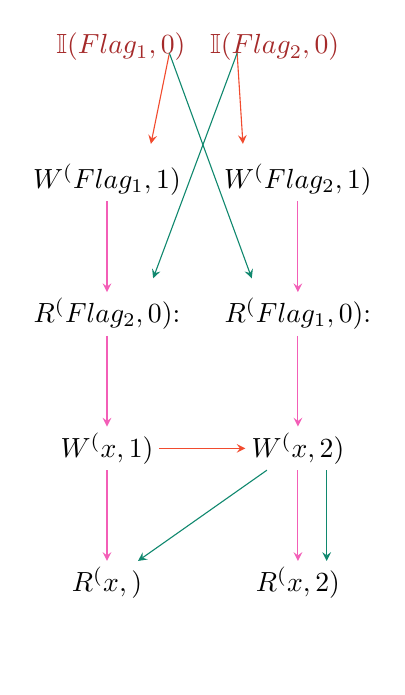
\begin{tikzpicture}[x=1em,y=1em,yscale=-1,xscale=-1]
	\tikzstyle{every node}=[font=\normalfont]
	
	\node (ifl1) [inner sep=2pt,color=Brown] {$\mathbb{I}(Flag_1,0)$};
	\node (ifl2) [right=30pt,inner sep=2pt,color=Brown] {$\mathbb{I}(Flag_2,0)$};
	
	\node (f11) [below left=10pt and -30pt of ifl1,inner sep=2pt, color=White] {$\mathbb{F}_{11}$};
	\node (fl1) [below=10pt of f11, inner sep=2pt] {$ W^\rlx(Flag_1,1) $};
	\node (f12) [below=10pt of fl1, inner sep=2pt, color=White] {$\mathbb{F}_{12}$};
	\node (rfl2) [below=10pt of f12, inner sep=2pt] {$R^\rlx(Flag_2,0)$:};
	\node (f13) [below=10pt of rfl2, inner sep=2pt, color=White] {$\mathbb{F}_{13}$};
	\node (cs11) [below=10pt of f13, inner sep=2pt] {$ W^\rlx(x,1) $};
	\node (f14) [below=10pt of cs11, inner sep=2pt, color=White] {$\mathbb{F}_{14}$};
	\node (cs12) [below=10pt of f14, inner sep=2pt] {$ R^\rlx(x,) $};
	\node (f15) [below=10pt of cs12, inner sep=2pt, color=White] {$\mathbb{F}_{15}$};
	
	\node (f21) [right=50pt of f11, inner sep=2pt, color=White] {$\mathbb{F}_{21}$};
	\node (fl2) [below=10pt of f21, inner sep=2pt] {$W^\rlx(Flag_2,1)$};
	\node (f22) [below=10pt of fl2, inner sep=2pt, color=White] {$\mathbb{F}_{22}$};
	\node (rfl1) [below=10pt of f22, inner sep=2pt] {$R^\rlx(Flag_1,0)$:};
	\node (f23) [below=10pt of rfl1, inner sep=2pt, color=White] {$\mathbb{F}_{23}$};
	\node (cs21) [below=10pt of f23, inner sep=2pt] {$ W^\rlx(x,2) $};
	\node (f24) [below=10pt of cs21, inner sep=2pt, color=White] {$\mathbb{F}_{24}$};
	\node (cs22) [below=10pt of f24, inner sep=2pt] {$ R^\rlx(x,2) $};
	\node (f25) [below=10pt of cs22, inner sep=2pt, color=White] {$\mathbb{F}_{23}$};
	%
	\draw [->,>=stealth,color=RedOrange] ($ (ifl1.south east)+(0.8,-5pt) $) -- node[pos=0.3,left=-2pt,font=\scriptsize,color=black] { $\lmo$ } ($ (fl1.north east)+(1.3,-5pt) $);
	\draw [->,>=stealth,color=RedOrange] ($ (ifl2.south west)+(-1.2,-5pt) $) -- node[pos=0.3,right=-2pt,font=\scriptsize,color=black] { $\lmo$ } ($ (fl2.north west)+(-0.9,-5pt) $);
	
	\draw [->,>=stealth,color=PineGreen] ($ (ifl1.south east)+(0.8,-5pt) $) -- node[pos=0.8,right=-2pt,font=\scriptsize,color=black] { $\lrf$ } ($ (rfl1.north west)+(-1.2,-5pt) $);
	\draw [->,>=stealth,color=PineGreen] ($ (ifl2.south west)+(-1.2,-5pt) $) -- node[pos=0.8,left=-2pt,font=\scriptsize,color=black] { $\lrf$ } ($ (rfl2.north east)+(1.2,-5pt) $);
	
	\draw [->,>=stealth,color=RedOrange] (cs11)  -- node[midway,above=-2pt,font=\scriptsize,color=black] { $\lmo$ } (cs21);
	\draw [->,>=stealth,color=PineGreen] (cs21)  -- node[midway,above=-2pt,font=\scriptsize,color=black] { $\lrf$ } (cs12);
	\draw [->,>=stealth,color=PineGreen] ($ (cs21.south)+(-10.4pt,0) $)  -- node[midway,right=-2pt,font=\scriptsize,color=black] { $\lrf$ } ($ (cs22.north)+(-10.4pt,0) $);
	
	\draw [->,>=stealth,color=CarnationPink] (fl1)  -- node[midway,right=-2pt,font=\scriptsize,color=black] { $\lsb$ } (rfl2);
	\draw [->,>=stealth,color=CarnationPink] (rfl2) -- node[midway,right=-2pt,font=\scriptsize,color=black] { $\lsb$ } (cs11);
	\draw [->,>=stealth,color=CarnationPink] (cs11) -- node[midway,right=-2pt,font=\scriptsize,color=black] { $\lsb$ } (cs12);
	
	\draw [->,>=stealth,color=CarnationPink] (fl2)  -- node[midway,right=-2pt,font=\scriptsize,color=black] { $\lsb$ } (rfl1);
	\draw [->,>=stealth,color=CarnationPink] (rfl1) -- node[midway,right=-2pt,font=\scriptsize,color=black] { $\lsb$ } (cs21);
	\draw [->,>=stealth,color=CarnationPink] (cs21) -- node[midway,right=-2pt,font=\scriptsize,color=black] { $\lsb$ } (cs22);
	
\end{tikzpicture}
} &
		\resizebox{0.24\textwidth}{!}{\tikzset{every picture/.style={line width=0.75pt}} %set default line width to 0.75pt        
\begin{tikzpicture}[x=1em,y=1em,yscale=-1,xscale=-1]
	\tikzstyle{every node}=[font=\normalfont]
	
	\node (ifl1) [inner sep=2pt,color=Brown] {$\mathbb{I}(Flag_1,0)$};
	\node (ifl2) [right=30pt,inner sep=2pt,color=Brown] {$\mathbb{I}(Flag_2,0)$};
	
	\node (f11) [below left=10pt and -30pt of ifl1,inner sep=2pt] {$\mathbb{F}_{11}$};
	\node (fl1) [below=10pt of f11, inner sep=2pt] {$ W^\sc(Flag_1,1) $};
	\node (f12) [below=10pt of fl1, inner sep=2pt] {$\mathbb{F}_{12}$};
	\node (rfl2) [below=10pt of f12, inner sep=2pt] {$R^\rlx(Flag_2,0)$:};
	\node (f13) [below=10pt of rfl2, inner sep=2pt] {$\mathbb{F}_{13}$};
	\node (cs11) [below=10pt of f13, inner sep=2pt] {$ W^\rlx(x,1) $};
	\node (f14) [below=10pt of cs11, inner sep=2pt] {$\mathbb{F}_{14}$};
	\node (cs12) [below=10pt of f14, inner sep=2pt] {$ R^\rlx(x,1) $};
	\node (f15) [below=10pt of cs12, inner sep=2pt] {$\mathbb{F}_{15}$};
	
	\node (f21) [right=50pt of f11, inner sep=2pt] {$\mathbb{F}_{21}$};
	\node (fl2) [below=10pt of f21, inner sep=2pt] {$W^\sc(Flag_2,1)$};
	\node (f22) [below=10pt of fl2, inner sep=2pt] {$\mathbb{F}_{22}$};
	\node (rfl1) [below=10pt of f22, inner sep=2pt] {$R^\rlx(Flag_1,0)$:};
	\node (f23) [below=10pt of rfl1, inner sep=2pt] {$\mathbb{F}_{23}$};
	\node (cs21) [below=10pt of f23, inner sep=2pt] {$ W^\rlx(x,2) $};
	\node (f24) [below=10pt of cs21, inner sep=2pt] {$\mathbb{F}_{24}$};
	\node (cs22) [below=10pt of f24, inner sep=2pt] {$ R^\rlx(x,1) $};
	\node (f25) [below=10pt of cs22, inner sep=2pt] {$\mathbb{F}_{23}$};
	%
	\draw [->,>=stealth,color=RedOrange] ($ (ifl1.south east)+(0.8,-5pt) $) -- node[pos=0.3,left=-2pt,font=\scriptsize,color=black] { $\lmo$ } ($ (fl1.north east)+(1.2,-5pt) $);
	\draw [->,>=stealth,color=RedOrange] ($ (ifl2.south west)+(-1.2,-5pt) $) -- node[pos=0.3,right=-2pt,font=\scriptsize,color=black] { $\lmo$ } ($ (fl2.north west)+(-0.7,-5pt) $);
	
	\draw [->,>=stealth,color=PineGreen] ($ (ifl1.south east)+(0.8,-5pt) $) -- node[pos=0.8,right=-2pt,font=\scriptsize,color=black] { $\lrf$ } ($ (rfl1.north west)+(-1.2,-5pt) $);
	\draw [->,>=stealth,color=PineGreen] ($ (ifl2.south west)+(-1.2,-5pt) $) -- node[pos=0.8,left=-2pt,font=\scriptsize,color=black] { $\lrf$ } ($ (rfl2.north east)+(1.2,-5pt) $);
	
	\draw [->,>=stealth,color=RedOrange] (cs11)  -- node[midway,above=-2pt,font=\scriptsize,color=black] { $\lmo$ } (cs21);
	\draw [->,>=stealth,color=PineGreen] (cs21)  -- node[midway,above=-2pt,font=\scriptsize,color=black] { $\lrf$ } (cs12);
	\draw [->,>=stealth,color=PineGreen] ($ (cs21.south)+(-10.4pt,0) $)  -- node[midway,right=-2pt,font=\scriptsize,color=black] { $\lrf$ } ($ (cs22.north)+(-10.4pt,0) $);
	
	\draw [->,>=stealth,color=CarnationPink] (f11)  -- node[midway,right=-2pt,font=\scriptsize,color=black] { $\lsb$ } (fl1);
	\draw [->,>=stealth,color=CarnationPink] (fl1)  -- node[midway,right=-2pt,font=\scriptsize,color=black] { $\lsb$ } (f12);
	\draw [->,>=stealth,color=CarnationPink] (f12)  -- node[midway,right=-2pt,font=\scriptsize,color=black] { $\lsb$ } (rfl2);
	\draw [->,>=stealth,color=CarnationPink] (rfl2) -- node[midway,right=-2pt,font=\scriptsize,color=black] { $\lsb$ } (f13);
	\draw [->,>=stealth,color=CarnationPink] (f13)  -- node[midway,right=-2pt,font=\scriptsize,color=black] { $\lsb$ } (cs11);
	\draw [->,>=stealth,color=CarnationPink] (cs11) -- node[midway,right=-2pt,font=\scriptsize,color=black] { $\lsb$ } (f14);
	\draw [->,>=stealth,color=CarnationPink] (f14)  -- node[midway,right=-2pt,font=\scriptsize,color=black] { $\lsb$ } (cs12);
	\draw [->,>=stealth,color=CarnationPink] (cs12) -- node[midway,right=-2pt,font=\scriptsize,color=black] { $\lsb$ } (f15);
	
	\draw [->,>=stealth,color=CarnationPink] (f21)  -- node[midway,right=-2pt,font=\scriptsize,color=black] { $\lsb$ } (fl2);
	\draw [->,>=stealth,color=CarnationPink] (fl2)  -- node[midway,right=-2pt,font=\scriptsize,color=black] { $\lsb$ } (f22);
	\draw [->,>=stealth,color=CarnationPink] (f22)  -- node[midway,right=-2pt,font=\scriptsize,color=black] { $\lsb$ } (rfl1);
	\draw [->,>=stealth,color=CarnationPink] (rfl1) -- node[midway,right=-2pt,font=\scriptsize,color=black] { $\lsb$ } (f23);
	\draw [->,>=stealth,color=CarnationPink] (f23)  -- node[midway,right=-2pt,font=\scriptsize,color=black] { $\lsb$ } (cs21);
	\draw [->,>=stealth,color=CarnationPink] (cs21) -- node[midway,right=-2pt,font=\scriptsize,color=black] { $\lsb$ } (f24);
	\draw [->,>=stealth,color=CarnationPink] (f24)  -- node[midway,right=-2pt,font=\scriptsize,color=black] { $\lsb$ } (cs22);
	\draw [->,>=stealth,color=CarnationPink] (cs22) -- node[midway,right=-2pt,font=\scriptsize,color=black] { $\lsb$ } (f25);
	
\end{tikzpicture}
} \\
		\hline
		
		\multicolumn{1}{c}{\hl{mutex-bt1}} &
		\multicolumn{1}{c}{$\imm{\hl{mutex-bt1}}$}  &
		\multicolumn{1}{c}{\hl{mutex-bt2}} &
		\multicolumn{1}{c}{$\imm{\hl{mutex-bt2}}$} \\
		
		\multicolumn{1}{c}{buggy trace 1} &
		\multicolumn{1}{c}{intermediate} &
		\multicolumn{1}{c}{buggy trace 2} &
		\multicolumn{1}{c}{intermediate} \\
	
		\multicolumn{1}{c}{} &
		\multicolumn{1}{c}{buggy trace 1} &
		\multicolumn{1}{c}{} &
		\multicolumn{1}{c}{buggy trace 2} \\
	\end{tabular}
\end{figure}

Algorithm~\ref{alg:main algo} iterates over each buggy trace
$\tau$ (line 4) and transforms the trace to an intermediate 
trace $\imm{\tau}$ (line 5). The algorithm further updates the 
event relations accordingly (line 6). As discussed in Section
\ref{sec:invalidating ce} a change is witnessed in the 
$\setHB$ relation. The transformed intermediate traces 
corresponding to buggy traces \hlref{mutex-bt1} and 
\hlref{mutex-bt2}, along with the updated event relations are 
represented in $\imm{\hlref{mutex-bt1}}$ and 
$\imm{\hlref{mutex-bt2}}$ respectively.

\noindent
{\bf Detecting cyclic relations indicating violation of 
	trace coherence}
In each intermediate buggy trace, the algorithm proceeds 
to perform \wkfence (line 7) and return cycles in compositions 
of event relations that define a coherence condition 
(Section~\ref{sec:c11}). For the intermediate traces 
$\imm{\hlref{mutex-bt1}}$ and $\imm{\hlref{mutex-bt2}}$
\wkfence would return an empty set.
%
The algorithm then proceeds to perform \stfence (line 8) that 
computes the $\so{\imm{\tau}}{}{}$ relation on \sc 
events and returns the cycles in $\so{\imm{\tau}}{}{}$.
The cyclic $\so{\imm{\tau}}{}{}$ relations in the intermediate
traces $\imm{\hlref{mutex-bt1}}$ and $\imm{\hlref{mutex-bt2}}$
are shown in $\imm{\hlref{mutex-bt1-so}}$ and 
$\imm{\hlref{mutex-bt2-so}}$. Note that, $\so{\imm{\tau}}{}{}$ 
would also be formed between every fence before 
$\mathbb{F}^\sc_{13}$ and every fence including and after 
$\mathbb{F}^\sc_{24}$ in $\imm{\hlref{mutex-bt1-so}}$ 
(correspondingly in $\imm{\hlref{mutex-bt1-so}}$), however, we 
have skipped the edges in the figures for better readability.

\begin{figure}[!h]
	\begin{tabular}{|c|c|}
		\hline
		\resizebox{0.24\textwidth}{!}{\tikzset{every picture/.style={line width=0.75pt}} %set default line width to 0.75pt        
\begin{tikzpicture}[x=1em,y=1em,yscale=-1,xscale=-1]
	\tikzstyle{every node}=[font=\normalfont]
	
	\node (ifl1) [inner sep=2pt,color=Brown] {$\mathbb{I}(Flag_1,0)$};
	\node (ifl2) [right=30pt,inner sep=2pt,color=Brown] {$\mathbb{I}(Flag_2,0)$};
	
	\node (f11) [below left=10pt and -30pt of ifl1,inner sep=2pt] {$\mathbb{F}^\sc_{11}$};
	\node (fl1) [below=10pt of f11, inner sep=2pt] {$ W^\sc(Flag_1,1) $};
	\node (f12) [below=10pt of fl1, inner sep=2pt] {$\mathbb{F}^\sc_{12}$};
	\node (rfl2) [below=10pt of f12, inner sep=2pt] {$R^\rlx(Flag_2,0)$:};
	\node (f13) [below=10pt of rfl2, inner sep=2pt] {$\mathbb{F}^\sc_{13}$};
	\node (cs11) [below=10pt of f13, inner sep=2pt] {$ W^\rlx(x,1) $};
	\node (f14) [below=10pt of cs11, inner sep=2pt] {$\mathbb{F}^\sc_{14}$};
	\node (cs12) [below=10pt of f14, inner sep=2pt] {$ R^\rlx(x,1) $};
	\node (f15) [below=10pt of cs12, inner sep=2pt] {$\mathbb{F}^\sc_{15}$};
	
	\node (f21) [right=50pt of f11, inner sep=2pt] {$\mathbb{F}^\sc_{21}$};
	\node (fl2) [below=10pt of f21, inner sep=2pt] {$W^\sc(Flag_2,1)$};
	\node (f22) [below=10pt of fl2, inner sep=2pt] {$\mathbb{F}^\sc_{22}$};
	\node (rfl1) [below=10pt of f22, inner sep=2pt] {$R^\rlx(Flag_1,0)$:};
	\node (f23) [below=10pt of rfl1, inner sep=2pt] {$\mathbb{F}^\sc_{23}$};
	\node (cs21) [below=10pt of f23, inner sep=2pt] {$ W^\rlx(x,2) $};
	\node (f24) [below=10pt of cs21, inner sep=2pt] {$\mathbb{F}^\sc_{24}$};
	\node (cs22) [below=10pt of f24, inner sep=2pt] {$ R^\rlx(x,1) $};
	\node (f25) [below=10pt of cs22, inner sep=2pt] {$\mathbb{F}^\sc_{23}$};
	%
	
	\draw [->,>=stealth,color=Mahogany] (f11)  -- node[pos=0.2,right=-2pt,font=\scriptsize,color=black] { $\lso$ } (f12);
	\draw [->,>=stealth,color=Mahogany] (f12)  -- node[pos=0.2,right=-2pt,font=\scriptsize,color=black] { $\lso$ } (f13);
	\draw [->,>=stealth,color=Mahogany] (f13)  -- node[pos=0.2,right=-2pt,font=\scriptsize,color=black] { $\lso$ } (f14);
	\draw [->,>=stealth,color=Mahogany] (f14)  -- node[pos=0.2,right=-2pt,font=\scriptsize,color=black] { $\lso$ } (f15);
	
	\draw [->,>=stealth,color=Mahogany] (f21)  -- node[pos=0.2,right=-2pt,font=\scriptsize,color=black] { $\lso$ } (f22);
	\draw [->,>=stealth,color=Mahogany] (f22)  -- node[pos=0.2,right=-2pt,font=\scriptsize,color=black] { $\lso$ } (f23);
	\draw [->,>=stealth,color=Mahogany] (f23)  -- node[pos=0.2,right=-2pt,font=\scriptsize,color=black] { $\lso$ } (f24);
	\draw [->,>=stealth,color=Mahogany] (f24)  -- node[pos=0.2,right=-2pt,font=\scriptsize,color=black] { $\lso$ } (f25);
	
	\draw [->,>=stealth,color=Mahogany] ($ (f12.north east) $)  to[out=-165,in=-15] node[midway,above=-2pt,font=\scriptsize,color=black] { $\lso$ } ($ (f22.north west) $);
	\draw [->,>=stealth,color=Mahogany] ($(f22.south west)$)  to[out=15,in=165] node[midway,below=-2pt,font=\scriptsize,color=black] { $\lso$ } ($(f12.south east)$);
	
	\draw [->,>=stealth,color=Mahogany] (f13)  -- node[midway,above=-2pt,font=\scriptsize,color=black] { $\lso$ } (f24);
	\draw [->,>=stealth,color=Mahogany] ($(f13.south east)$)  to[out=155,in=0] node[midway,left=-2pt,font=\scriptsize,color=black] { $\lso$ } ($(f25.west)$);
	
\end{tikzpicture}
} &
		\resizebox{0.24\textwidth}{!}{\tikzset{every picture/.style={line width=0.75pt}} %set default line width to 0.75pt        
\begin{tikzpicture}[x=1em,y=1em,yscale=-1,xscale=-1]
	\tikzstyle{every node}=[font=\normalfont]
	
	\node (ifl1) [inner sep=2pt,color=Brown] {$\mathbb{I}(Flag_1,0)$};
	\node (ifl2) [right=30pt,inner sep=2pt,color=Brown] {$\mathbb{I}(Flag_2,0)$};
	
	\node (f11) [below left=10pt and -30pt of ifl1,inner sep=2pt] {$\mathbb{F}^\sc_{11}$};
	\node (fl1) [below=10pt of f11, inner sep=2pt] {$ W^\sc(Flag_1,1) $};
	\node (f12) [below=10pt of fl1, inner sep=2pt] {$\mathbb{F}^\sc_{12}$};
	\node (rfl2) [below=10pt of f12, inner sep=2pt] {$R^\rlx(Flag_2,0)$:};
	\node (f13) [below=10pt of rfl2, inner sep=2pt] {$\mathbb{F}^\sc_{13}$};
	\node (cs11) [below=10pt of f13, inner sep=2pt] {$ W^\rlx(x,1) $};
	\node (f14) [below=10pt of cs11, inner sep=2pt] {$\mathbb{F}^\sc_{14}$};
	\node (cs12) [below=10pt of f14, inner sep=2pt] {$ R^\rlx(x,1) $};
	\node (f15) [below=10pt of cs12, inner sep=2pt] {$\mathbb{F}^\sc_{15}$};
	
	\node (f21) [right=50pt of f11, inner sep=2pt] {$\mathbb{F}^\sc_{21}$};
	\node (fl2) [below=10pt of f21, inner sep=2pt] {$W^\sc(Flag_2,1)$};
	\node (f22) [below=10pt of fl2, inner sep=2pt] {$\mathbb{F}^\sc_{22}$};
	\node (rfl1) [below=10pt of f22, inner sep=2pt] {$R^\rlx(Flag_1,0)$:};
	\node (f23) [below=10pt of rfl1, inner sep=2pt] {$\mathbb{F}^\sc_{23}$};
	\node (cs21) [below=10pt of f23, inner sep=2pt] {$ W^\rlx(x,2) $};
	\node (f24) [below=10pt of cs21, inner sep=2pt] {$\mathbb{F}^\sc_{24}$};
	\node (cs22) [below=10pt of f24, inner sep=2pt] {$ R^\rlx(x,1) $};
	\node (f25) [below=10pt of cs22, inner sep=2pt] {$\mathbb{F}^\sc_{23}$};
	%
	
	\draw [->,>=stealth,color=Mahogany] (f11)  -- node[pos=0.2,right=-2pt,font=\scriptsize,color=black] { $\lso$ } (f12);
	\draw [->,>=stealth,color=Mahogany] (f12)  -- node[pos=0.2,right=-2pt,font=\scriptsize,color=black] { $\lso$ } (f13);
	\draw [->,>=stealth,color=Mahogany] (f13)  -- node[pos=0.2,right=-2pt,font=\scriptsize,color=black] { $\lso$ } (f14);
	\draw [->,>=stealth,color=Mahogany] (f14)  -- node[pos=0.2,right=-2pt,font=\scriptsize,color=black] { $\lso$ } (f15);
	
	\draw [->,>=stealth,color=Mahogany] (f21)  -- node[pos=0.2,right=-2pt,font=\scriptsize,color=black] { $\lso$ } (f22);
	\draw [->,>=stealth,color=Mahogany] (f22)  -- node[pos=0.2,right=-2pt,font=\scriptsize,color=black] { $\lso$ } (f23);
	\draw [->,>=stealth,color=Mahogany] (f23)  -- node[pos=0.2,right=-2pt,font=\scriptsize,color=black] { $\lso$ } (f24);
	\draw [->,>=stealth,color=Mahogany] (f24)  -- node[pos=0.2,right=-2pt,font=\scriptsize,color=black] { $\lso$ } (f25);
	
	\draw [->,>=stealth,color=Mahogany] ($ (f12.north east) $)  to[out=-165,in=-15] node[midway,above=-2pt,font=\scriptsize,color=black] { $\lso$ } ($ (f22.north west) $);
	\draw [->,>=stealth,color=Mahogany] ($(f22.south west)$)  to[out=15,in=165] node[midway,below=-2pt,font=\scriptsize,color=black] { $\lso$ } ($(f12.south east)$);
	
	\draw [->,>=stealth,color=Mahogany] (f23)  -- node[midway,above=-2pt,font=\scriptsize,color=black] { $\lso$ } (f14);
	\draw [->,>=stealth,color=Mahogany] ($(f23.south west)$)  to[out=25,in=180] node[midway,right=-2pt,font=\scriptsize,color=black] { $\lso$ } ($(f15.east)$);
	
\end{tikzpicture}
} \\
		\hline
		
		\multicolumn{1}{c}{$\imm{\hl{mutex-bt1-so}}$}  &
		\multicolumn{1}{c}{$\imm{\hl{mutex-bt2-so}}$-} \\
		
		\multicolumn{1}{c}{intermediate} &
		\multicolumn{1}{c}{intermediate} \\
		
		\multicolumn{1}{c}{buggy trace 1} &
		\multicolumn{1}{c}{buggy trace 2} \\
	\end{tabular}
\end{figure}


\subsection{Reducing Fence Synthesis to SAT problem}
Recall that transitive closure of $ \so{\imm{\tau}}{}{} $ is same as 
$ \to{\imm{\tau}}{}{} $ in a valid \cc trace. Since  
$ \to{\imm{\tau}}{}{} $ is a total order, a valid \cc trace should not 
have a cycle in $ \so{\imm{\tau}}{}{} $. Conversely, if a trace has 
$ \so{\imm{\tau}}{}{} $-cycle, it cannot be a valid \cc trace. 
In order to make a trace $ \tau $ invalid under \cc, we force a \lso-cycle by inserting appropriate fences. 
Since $ \imm{\tau} $ assumes \mosc fences at all possible program locations,
any such cycle must exists in $ \so{\imm{\tau}}{}{} $. 
Hence, our problem is reduced to finding appropriate cycle in 
$\so{\imm{\tau}}{}{} $ and introducing these fences in the program to 
invalidate the trace $ \tau $.
If we introduced enough fences to cause at least \lso-cycle in 
every counter example, we stop all the buggy trace. 
It is possible that a counter example $ \tau $ does not have any 
$\so{\imm{\tau}}{}{}$-cycles. Since $ \imm{\tau} $ has \mosc fences at all 
possible program locations, we cannot add fences in such a trace to 
make it invalid \cc trace. 
Line 8 in Algorithm~\ref{alg:fence-syn} computes set $\so{\imm{\tau}}{}{}$-cycles. 
The problem of finding cycles in a graph is well-studied area. Hence, we 
choose to skip the details of this step.
If there are no $\so{\imm{\tau}}{}{}$-cycle in some $ \tau $, we conclude 
that it is not possible to stop this trace using \cc fences in lines 
9-11.


Let $ \cycles{\imm{\tau}} $ be the set of \lso-cycles in a trace $ \imm{\tau} $, 
where a cycle $ c \in \cycles{\imm{\tau}} $ is ordered sequence of 
$ \ordevents{\sc} $. We abuse the notation $\ordevents{\sc}_c$ to 
represent the set of events in a cycle $ c $. 
All the read and write events in $\ordevents{\sc}_c$ are already in program $ P $. 
Hence, to introduce a cycle $ c $ in the trace, we add the fences in $\ordevents{\sc}_c$, i.e, 
$\ordfences{\sc}_c$, in the program $ P $.
In other words, a cycle $ c $ can be introduced in a program if we insert 
$ (\bigwedge\limits_{f \in \ordfences{\sc}_c} f)$ fences in the program $ P $, 
where the truth assignment to a fence corresponds to inserting that fence 
in the program.
Recall that we need to stop at least one cycle from the set 
$ \cycles{\imm{\tau}} $ in order to make a trace $ \tau $ invalid.
Hence we need to insert $ (\bigvee\limits_{c \in \cycles{\imm{\tau}}} (\bigwedge\limits_{\fn{} \in \ordevents{\sc}_c \intersection 
\ordfences{\sc}} \fn{})) $ to stop a trace $ \tau $. 
We use $\formula{\so{\imm{\tau}}{}{}}$ to represent the boolean formula 
corresponding to the $ \so{\imm{\tau}}{}{} $-cycles.
Clearly, any satisfying assignment to $ \formula{\so{\imm{\tau}}{}{}} $ 
will give list of fences required to stop the buggy trace $ \tau $.
%
Furthermore, we construct the formula for all trace 
$ \tau \in \mathcal{CE} $ by conjuncting them in 
line 12 of Algorithm~\ref{alg:fence-syn}, i.e., 
at the end of the for loop in lines 4-12, the formula 
$ \phi \definedas (\bigwedge\limits_{\tau \in \mathcal{CE}} 
(\bigvee\limits_{c \in \cycles{\imm{\tau}}} 
(\bigwedge\limits_{\fn{} \in \ordevents{\sc}_c \intersection \ordfences{\sc}} \fn{}))) $.
Any satisfying assignment of the formula $\phi$ will list the fences that 
are enough to stop the buggy traces in $ \mathcal{CE} $.

%\begin{lemma}
%	Introducing fences in any $\so{\imm{\tau}}{}{}$-cycle will stop the counter example $ \tau $ in actual trace of the program.
%\end{lemma}

\begin{lemma}
	If there are no cycles in $\so{\imm{\tau}}{}{}$ of a buggy trace 
	$\tau$, the counter-example $ \tau $ cannot be stopped using any \cc 
	fences.
\end{lemma}

\begin{theorem}
	Any satisfying assignment to $ \formula{\so{\imm{\tau}}{}{}} $ 
	will give list of fences required to stop the buggy trace $ \tau $
\end{theorem}


\subsection{Finding Optimal Placement of the Fences}
One possible satisfying assignment to formula $ \phi $ is assigning the 
value true to all fences. Clearly such a solution is very expensive.
The number of truth assignments in the solution of formula $ \phi $ is 
equal to the number of fences inserted in the program.
%A satisfying assignment of the formula $ \phi $ with lesser number 
%of fences will give us a more optimal fence placement. 
Hence, a satisfying assignment of the formula $ \phi $ with the least 
number of fences will give us the optimal fence placement. 
Therefore, we reduce the problem of finding optimal fence placement to the 
minimal model of a SAT formula. 

The problem of minimal model computation has been studied in 
\divComment{need references}. \divComment{Need complexity argument for min model}.

In some cases, a fence at certain program location maybe more expensive 
than at other program location. For example, a fence inside a loop is may 
execute several times. Hence, such a fence may be more expensive than a 
fence placed outside the loop body.
%
\ourtechnique can handle such constraints by using weighted minimal model 
problem \divComment{need references}, where weight of each fence 
corresponds how expensive the fence is. 
The Algorithm~\ref{alg:fence-syn} can be modified to take weight 
function as input. 
%
The current implementation of \ourtechnique uses repeated calls to Z3 SAT 
solver to find the minimal model. \divComment{How are we solving it?}


\begin{theorem}
	For any input program $ P $, minimal model of $ \phi $ gives optimal
	number of fences required to stop all the buggy traces in 
	$ \mathcal{CE} $.
\end{theorem}



\section{Technical Implementation/Tool Description}
\par
The tool is created using the python programming language. Extra libraries used:
\begin{itemize}
	\item networkx - for graphing related queries, such as find cycles
	\item ast - for evaluating values from store
	\item operator
	\item shlex
	\item argparse
	\item os
\end{itemize}

\subsection{Translating model checker output}
The tool begins by translating model checker output that it obtains from the terminal process after running the required command. From CDS Checker output, it extracts the following information for each instruction in the trace:
\begin{enumerate}
	\item thread number of the instruction
	\item instruction type (thread create, thread start, init, atomic read, atomic write, atomic rmw)
	\item memory order (relaxed, acquire, release, acq\textunderscore rel, seq\textunderscore cst)
	\item memory address (variable name in the system)
	\item value
	\item rf value (in case of read/rmw instruction)
\end{enumerate}

\par 
Other required information is extracted from the C++ source program. These include:
\begin{enumerate}[7.]
	\item variable name for each instruction
	\item line number for each instruction
\end{enumerate}

\par
For any of the above meta-data, if a field does not apply for a certain instruction, it is given the value "NA".

\subsubsection{Extracting line numbers}
Line numbers are extracted by pattern-matching the instruction meta-data in the above mentioned fields, creating the instruction out of them and matching them to the source thread. For example, the information extracted for a single instruction is: thread number 2, instruction type read, memory order seq\_ cst, memory address \textit{x}. Then the instruction would be created as \texttt{x.load(memory\_ order\_ seq\_ cst)} and be matched inside the function defined for thread 2. There are also contingencies for this procedure, so certain rules need to be followed in the input program.

\par
Since line numbers are required to be extracted from the source program in order to obtain the locations where the fences need to be inserted, the source program needs to follow a certain structure for the tool to work. The rules are:
\begin{enumerate}
	\item Each atomic operation needs to be on a separate line.\\
	\textit{Example:} \texttt{a.store(b.load(memory\_ order\_ relaxed), memory\_ order\_ relaxed));} needs to be re-written as the following snippet:\\
	\texttt{%
	int temp = b.load(memory\_ order\_ relaxed);\\
	a.store(temp, memory\_ order\_ relaxed));%
	}
	unless it is an argument inside (say) an if statement with boolean operators like \texttt{if(a.load(memory\_ order\_ relaxed) || b.load(memory\_ order\_ relaxed)) }\\
	This is because each atomic access is treated as a separate entity in the model checker's output.
	
	\item Each atomic variable used in the program needs to be initialized in the main/parent thread. The tool maps the variable name to its memory address through the initialized values.
	
	\item While writing a "store" operation, there needs to be a space character after the comma after the value is written.\\
	\textit{Example:} \texttt{a.store(0, memory\_ order\_ relaxed)} and not \texttt{a.store(0,memory\_ order\_ relaxed)}
	
	\item The thread functions need to be defined in the same order as they were called in the main/parent thread before the main thread and there can be no other extra functions apart from the thread functions and the main function.
	
	\item The starting bracket for each function definition, loop call, or if-else statement needs to be in the same line as the function name.\\
	\textit{Example:} \texttt{static void t1() \{} and not\\ \texttt{static void t1()\\ \{}
	
	\item \textbf{\textit{Handing RMW instructions:}} since RMW instructions can be of any type (such as fetch\_ add, fetch\_ sub, etc) and still be just referred to as "atomic rmw" in the model checker, it can be hard to pattern-match these lines. Therefore another technique is used for pattern matching here. A "dummy variable" is created and a "store" operation is added to the line right above the RMW instruction. The value that it is storing needs to differ each time it is called in order to maintain uniqueness. Then the tool simply pattern-matches the instruction right above the RMW in the given thread and finds the line by adding "1" to the line number of the dummy variable store operation.\\
	\textit{Example:}\\ \texttt{[14] dummy.store(2, memory\_ order\_ relaxed);}\\ \texttt{[15] x.fetch\_ xor(1, memory\_ order\_ acq\_ rel);}\\
	This method also does not hinder the flow of the program since the operation on the dummy variable is a store operation which is never read, hence never forming an rf relation. The memory order will also never be "seq\_ cst", so it will never be considered while calculating TO relations.
	
	\item The above method is also to be used every time there is a repeated instruction in the same thread. For example if the instruction \texttt{b.load(memory\_ order\_ relaxed);} is called twice inside a single thread, pattern-matching this line would not be able to point to the instruction which called it at that point. Therefore, a dummy store operation needs to be inserted above every one of these repeating operations.\\\textit{Note:} only if the exact instruction matches does the dummy method need to be applied. If the memory orders or store values are different, then the instructions become different.
	
	% also add dummy variable store operation above a store instruction whose valule is another variable like a.store(temp, mo_relaxed); since "temp" will not be given by CDS Checker and only the value can be matched.
	
	\item "thread create" statements inside loops need to be unravelled and their functions need to be re-written as many times as they are called, with different names. This is because if there are multiple thread spawns from the a function using a loop, the number of threads will differ for each trace in the model checker. The model checker will treat them as different thread functions instead of the same one being called. Moreover, there might be cases where fences need to be inserted in the thread in one of the iterations of the loop but not the other.\\
	\textit{Example:}\\ \texttt{%
	static void thread1();\\
	int main() \{\\
	\hspace{10mm} for(3 iterations) \{\\
	thread\_ create(thread1);\\
	\}\}%
	}\\ needs to be re-written as:\\
	\texttt{%
	static void thread1();\\
	static void thread2();\\
	static void thread3();\\
	int main() \{\\
	thread\_ create(thread1);\\
	thread\_ create(thread2);\\
	thread\_ create(thread3);\\
	\}%
	}
	
	\item 'IF' and 'FOR' statements always need to be bracketed in case there is a fence insertion taking place inside.
\end{enumerate}


\bibliographystyle{unsrtnat}
\bibliography{References.bib}
\end{document}
